\chapter{SMTP, IMAP szerver}

\section{hMailServer}
\begin{flushleft}
    Be kell kapcsolni az SMTP, IMAP protokollokat, ezután meg kell adni a megfelelő domain nevét: \verb|oemail.io|. Itt hozhatunk létre IMAP fiókokat is, amit az \verb|Accounts| menüpontban tehetünk meg.
    \begin{center}
        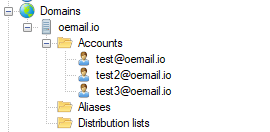
\includegraphics[width=0.5\textwidth]{hmailServer-accounts.png}
    \end{center}
\end{flushleft}

\section{Alapértelmezett mappák}
\begin{flushleft}
    Új fiók regisztrációja során az alábbi mappák kerülnek létrehozásra:
    \begin{itemize}
        \item \textbf{INBOX}: Bejövő emailek.
        \item \textbf{SENT}: Elküldött emailek.
        \item \textbf{TRASH}: Szemét, törölt emailek.
        \item \textbf{SPAM}: Gyanús emailek.
        \item \textbf{STARS}: Kedvenc emailek.
    \end{itemize}
\end{flushleft}